\documentclass{jsarticle}
\usepackage{amssymb,amsmath}
\usepackage{amsthm}
\usepackage{newtxtt}
\usepackage[dvipdfmx]{graphicx}
\usepackage{tikz}
\usepackage[utf8]{inputenc}
\newtheorem{th.}{Statement}
\newcommand{\pder}[2][]{\frac{\partial#1}{\partial#2}}
\newcommand{\dder}[2][]{\frac{\mathrm{d}#1}{\mathrm{d}#2}}
\newcommand{\ppder}[2][]{\frac{\partial^2#1}{{\partial#2}^2}}
\newcommand{\pikder}[3][]{\frac{\partial^2#1}{{\partial#2 \partial#3}}}
\newcommand{\pikdergx}[3][]{\frac{\partial^2 g_{#1}}{{\partial x^{#2} \partial x^{#3}}}}
\newcommand{\pderx}[2][]{\pder[#1]{x^{#2}}}
\newcommand{\pdergx}[2][]{\pderx[g_{#1}]{#2}}
\newcommand{\half}{\frac{1}{2}}
\newcommand{\hfpt}{\hspace{5pt}}
\newcommand{\ddfrac}[2]{\frac{{#1}^2}{{#2}^2}}
\newcommand{\beq}{\begin{equation}}
\newcommand{\beql}[1]{\begin{equation}\label{#1}}
\newcommand{\eeq}{\end{equation}}
\newcommand{\eeqp}{\;\;\;.\end{equation}}
\newcommand{\eeqc}{\;\;\;,\end{equation}}
\newcommand{\GaT}[3]{\Gamma^{#1}_{#2 #3}}
\newcommand{\pderGaTx}[4]{\pderx[\GaT{#1}{#2}{#3}]{#4}}
\newcommand{\Christfinside}[3]{\pdergx[#3 #1]{#2} + \pdergx[#2 #3]{#1} - \pdergx[#1 #2]{#3}}
\newcommand{\Christf}[4]{\Gamma^{#1}_{#2 #3}=\half g^{#1 #4}(\Christfinside{#2}{#3}{#4})}
\newcommand{\Ricchiinside}[2]{\pder[\Gamma^l_{#1 #2}]{x^l} - \pder[\Gamma^l_{#1 l}]{x^{#2}} 
    + \GaT{l}{#1}{#2}\GaT{m}{l}{m} - \GaT{m}{#1}{l}\GaT{l}{#2}{m}}
\date{\today}
\author{山田龍}
\title{フレネル積分}
\begin{document}
\maketitle
\section{}
\begin{th.}
    \beq
        \int_{0}^{\infty} \cos x^2 = 0
    \eeq
\end{th.}
\begin{flushright}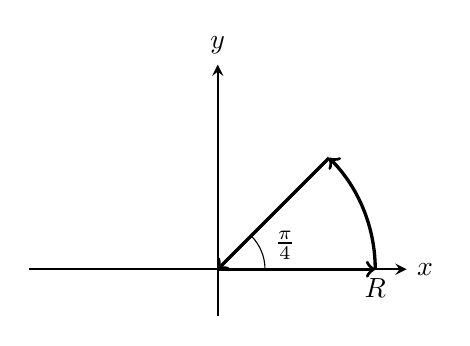
\begin{tikzpicture}[scale=2]
       %ここにTikZのコマンドを記述します。
     % 軸
    \draw[thick, -stealth] (-1.2, 0)--(1.2, 0) node[right] {$x$};
    \draw[thick, -stealth] (0, -0.3)--(0, 1.3) node[above] {$y$};
    \draw[very thick, ->] (1,0)arc (0:45:1);
    \draw[thin] (0.3,0)arc (0:45:0.3);
    \draw[very thick,->] (0,0)--(1,0);
    \draw[very thick,->] ({sqrt(1/2)},{sqrt(1/2)})--(0,0);
    \draw (1, 0) node[below] {$R$};
    \coordinate (thrta_0) at (0.3,0) node at (thrta_0) [above right] {$\frac{\pi}{4}$};%角度のラベル
\end{tikzpicture}\end{flushright}
$cos z^2$について考える。積分区間を$\frac{\pi}{4}$の扇形一周に取る。
\beq
    \int_C \cos z^2 = \int + \int + \int
\eeq
と書き換える。ここで、積分経路で囲まれた領域に特異点がないから、つまりどの点でもコーシーリーマンの関係式を満たすので左辺は0である。
\end{document}

